\chapter{Hešovanie: \vb{<unordered\_set>} a \vb{<unordered\_map>} v STL}
\label{sect:hesovanie}


Vráťme sa k úlohe~\ref{uloha:ziarovky-vela}. Opäť budeme mať žiarovky, ktoré
budú mať výrobné čísla \prg!unsigned long!, takže budú z rozsahu $0$ až $M-1$, 
kde $M=2^{64}$. Zároveň pre jednoduchší začiatok predpokladajme, že vieme, 
že budeme mať presne $n\ll M$ žiaroviek. Na vstupe budú  opäť chodiť príkazy na prepnutie
žiarovky a otázky, či nejaká žiarovka svieti. V kapitole \ref{sect:stromy} sme
to riešili použitím vyhľadávacích stromov. Teraz si ukážeme iný spôsob riešenia,
ktorému sa hovorí {\em hešovanie}.


Keby sme z nejakého dôvodu vedeli, že nám budú v nejakom poradí chodiť žiarovky
s číslami $42$, $43$, $44, \ldots, 41+n$, stačilo by rezervovať si pole \prg!bool A[n]!
a stav žiarovky s číslom $z$ by sme si mohli pamätať v premennej \prg!A[z-42]!. 
Podobne keby sme vedeli, že budú chodiť žiarovky $2,4,\ldots,2n$, tiež by stačilo rezervovať
pole  \prg!bool A[n]! a žiarovku s číslom $z$ by sme mali v premennej \prg!A[z/2-1]!.
V oboch prípadoch by sme mali nejakú funkciu \prg!int h(unsigned long z) { ... }!,
ktorá pre číslo žiarovky vyráta jej umiestnenie v poli, takže žiarovka $z$
je umiestnená v \prg!A[h(z)]!. Ideálne by bolo, keby som mohol mať
jednu takú funkciu \vb{h}, ktorá by fungovala pre viacero (ideálne pre všetky)
možné vstupy. Každú funkciu \vb{h}, bez ohľadu na to, ako sa vypočíta,
si viem predstaviť ako kartičku, kde pre každý z $M$ bodov v hornom riadku (všetky možné výrobné čísla)
ide šípka do nejakého bodu v spodnom riadku (všetky pozície v poli).

\centerline{
  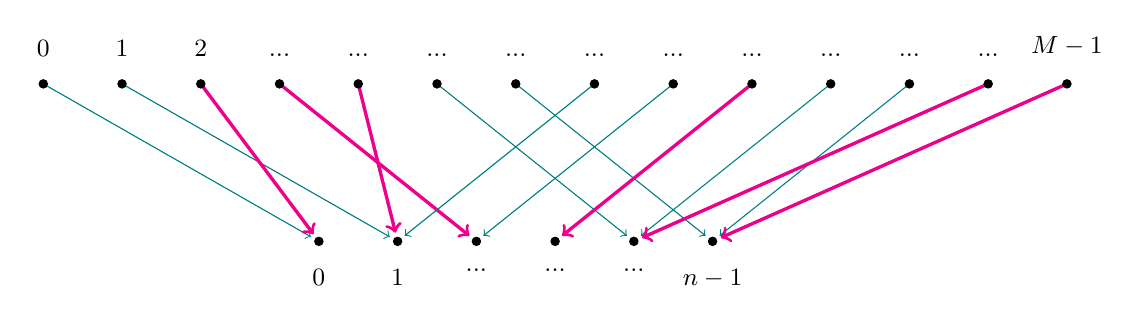
\begin{tikzpicture}
    \tikzstyle{sipkaA}= [teal,->,shorten >= 0.75ex]
    \tikzstyle{sipkaB}= [magenta, very thick,->,shorten >= 0.75ex]
  \def\dot(#1){\filldraw (#1) circle (1.5pt)}
  \def\hi{2}
  \def\M{13}
  \def\n{6}
  \pgfmathsetmacro{\lox}{(\M-\n)/2-1}

  \foreach \t/\s [count=\x] in {1/A,2/A,1/B,3/B,2/B,5/A,6/A,2/A,3/A,4/B,5/A,6/A,5/B,6/B} 
    \draw[sipka\s] (\x-1,\hi) -- (\t+\lox,0);

  \foreach \x in {0,...,\M}
    \dot(\x,\hi);

  \xdef\alist{0,1,2}
  \pgfmathtruncatemacro{\tmp}{\M-4}
  \foreach \i in {0,...,\tmp} {
    \xdef\alist{\alist, {...} }
  }
  \xdef\alist{\alist, M-1}
  \foreach \l [count=\x] in \alist
    \node[above,yshift=1.5ex] at (\x-1,\hi) {{\small$\l$}};
  
  \foreach \x in {1,...,\n}
    \dot(\x+\lox,0);

  \xdef\alist{0,1}
  \pgfmathtruncatemacro{\tmp}{\n-4}
  \foreach \i in {0,...,\tmp} {
    \xdef\alist{\alist, {...} }
  }
  \xdef\alist{\alist, n-1}
  \foreach \l [count=\x] in \alist
    \node[below,yshift=-1.5ex] at (\x+\lox,0) {{\small$\l$}};

\end{tikzpicture}}

Ak používam túto konkrétnu funkciu \vb{h}, tak
pri každom spustení sa na vstupe ocitne $n$ rôznych výrobných čísel (fialové šípky)
a o týchto chceme, aby sa zobrazili na rôzne miesta. Keď sa nad tým chvíľu zamyslíš,
tak je zrejmé, že to nemôže fungovať: nech sú šípky zoradené hocijako,
máme $M$ šípok a $n$ cieľov, preto musí
byť cieľ, do ktorého smeruje aspoň $M/n$ šípok. No a keďže $M$ je veľmi veľké, 
dá sa nájsť vstup, v ktorom všetkých $n$ vybratých
šípok ukazuje do tej istej pozície.

Napriek tomu, že je jasné, že to nebude fungovať, skúsme byť chvíľu tvrdohlaví
a pokračovať v úvahách. Dajme tomu, že by sme mali nejakú takúto {\em hešovaciu} funkciu \vb{h},
\indexItem{Alg}{hešovacia funkcia, kolízie}
teda nejak vybraté modré šípky. Podľa toho, ktoré
výrobné čísla sa objavia na vstupe, niektoré šípky budú fialové.
Nedúfame, že naša funkcia bude úplne dokonalá, a tak sa nám možno môže stať, že niekoľko
fialových šípok bude smerovať do rovnakého cieľa. Ak ich ale nebude veľa, 
ešte to nie je stratené. Takéto tzv. {\em kolízie} môžeme vyriešiť napr. tak,
že v našom poli \prg!A! si nebudeme na pozícii \prg!h(i)!
ukladať \prg!bool! hodnotu, či je žiarovka s číslom  \prg!h(i)! zapnutá, ale
spájaný zoznam zapnutých žiaroviek so všetkými výrobnými číslami $x$,
pre ktoré $\vb{h}(x)=\vb{h}(i)$. Môžme to naprogramovať napr. takto:


\label{pg:lst:hash}
\begin{lstlisting}
using Key = unsigned long;
using HashFunct = function<int(Key)>;
  
struct HashMap { 
  vector<forward_list<Key>> A;
  HashFunct h;
    
  HashMap(int n, HashFunct _h) : h{_h} { A.resize(n); }
  
  void insert(Key x) {
    auto &list = A[h(x)];
    if (find(list.begin(), list.end(), x) == list.end()) 
      list.push_front(x);
  } 
    
  void erase(Key x) {
    auto &list = A[h(x)];
    auto it = find(list.begin(), list.end(), x);
    if (it != list.end()) {
      *it = *list.begin();
      list.pop_front();
    }
  } 
  
  bool contains(Key x) {
    auto &list = A[h(x)];
    return find(list.begin(), list.end(), x) != list.end();
  }
};  
\end{lstlisting}

V tomto programe je hešovacia funkcia typu \prg!HashFunct!, t.j. dostane parameter $x$
a vráti hodnotu $h(x)$ z rozsahu $0,\ldots,n-1$. Premenná typu 
\prg!HashMap! dostane v konštruktore dĺžku poľa $n$ a hešovanciu funkciu, 
a potom má metódy \prg!insert!, \prg!erase! a \prg!contains!, ktoré sú zjavné.
Mohli by sme teda napísať
napr. \prg!HashMap h(10, [](Key x) { return x % 10; });!.
a po tom, čo postupne zavoláme \vb{insert} s hodnotami 
\vb{77 5 23 18 43 57 15 43 42 85 } to bude v pamäti vyzerať takto:\\


\centerline{\begin{tikzpicture}[scale=0.8]
  \def\h{0.35}
  \def\nodecolor{cyan!50!blue}
  \foreach \i in {0,...,9} {
  \draw(\i,0) rectangle (\i+1,2*\h);
  \node[above]at(\i+0.5,2*\h){$\i$};
  \fill[\nodecolor](\i+0.5,\h) coordinate (base\i)circle (0.1); 
  }
  \node[anchor=east]at(0,0.5){\vb{A}:};

  \def\zoz#1(#2,#3)#4{
    \begin{scope}[shift={($(#2,1.15*#3)+(0.5,0.5)$)}]
      \draw[\nodecolor,rounded corners=2pt](-0.4,-\h) rectangle (0.4,\h);
      \node[\nodecolor] at(0,0) {\vb{#4}};
      \coordinate (top#1) at (0,\h);
      \coordinate (bot#1) at (0,-\h);
      \fill[\nodecolor] (bot#1) circle (0.1);
  \end{scope}
  }

  \foreach \x/\l in {2/{4},3/{4,2},5/{8,1,{}},7/{5,7},8/{1}} {
    \foreach \val [count = \i, 
        remember = \c as \lastC (initially base\x)
    ] in \l {
        \zoz{\i}(\x,-\i){\val\x}
        \def\c{bot\i}      
        \draw[\nodecolor, ->] (\lastC) -- (top\i);
    }
  }

\end{tikzpicture}}


Akú by mal náš program zložitosť? Každá z funkcií \vb{insert}, \vb{erase}, \vb{contains}
najprv vyráta hešovaciu funkciu (nateraz predpokladajme, že to vieme urobiť rýchlo)
a potom v najhoršom prípade prehľadá celý spájaný zoznam \prg!A[h(x)]!. Takže zložitosť každej
operácie je úmerná dĺžke zoznamu \prg!A[h(x)]!. V zozname \prg!A[h(x)]! skončia všetky
žiarovky zo vstupu, ktorých výrobné číslo má v našej hešovacej funkcii kolíziu s výrobným
číslom $x$, t.j. žiarovky s číslom $z$, pre ktoré platí $\vb{h}(x)=\vb{h}(z)$,
preto zložitosť nášho programu bude závisieť od počtu kolízii našej hešovacej funkcie.


A sme zase tam, kde sme boli na začiatku: nech si zvolíme hocijakú hešovaciu funkciu,
vždy bude existovať vstup, na ktorom bude mať veľa kolízií. 
Opäť nám ale príde na pomoc náhoda. Na začiatku síce nevieme, aké výrobné čísla
budú na vstupe, ale ako funkciu \prg!h! si vyberieme náhodnú funkciu. Čo to znamená
náhodná funkcia? Funkcia je obrázok, kde z každého z $M$ výrobných čísel ide
modrá šípka do niektorého z $n$ miest. Koľko
je takých rôznych obrázkov? Na obrázku je $M$ šípok a každá z nich má $n$ možných cieľov,
teda dokopy je $n^M$ možností. Napíšeme si ich na papieriky a vložíme do vrecka.
Potom náhodne vytiahneme jeden obrázok a máme náhodnú funkciu.
Kontrolná otázka:

\begin{uloha}
  \label{uloha:nahprm}
  Vyberme si náhodnú funkciu \prg!h!. Aká je pravdepodobnosť, že $\vb{h}(42)=1$?
\end{uloha}

Vyšlo ti $1/n$? Dobre. Jedna možnosť, ako sa o tom presvedčiť, je pozrieť sa na
všetkých $n^M$ papierikov a ofarbiť ich podľa toho, aká je hodnota $\vb{h}(42)$:
ak  $\vb{h}(42)=0$, papierik bude modrý, ak  $\vb{h}(42)=1$, bude červený atď.
Vo vrecku teda budem mať papieriky $n$ farieb. Koľko je tam papierikov jednej farby?
Bez ohľadu na to, kam smeruje šípka $\vb{h}(42)$, ostatné šípky sú umiestené hocijako,
a teda mám $n^{M-1}$ možností. Pôvodnú úlohu sa teraz
viem opýtať takto: vo vrecku mám $n^M$ papierikov ofarbených $n$ farbami, 
pričom z každej farby mám rovnako veľa, t.j. $n^{M-1}$ papierikov.
Aká je pravdepodobnosť, že vytiahnem červený papierik? Tu je ale odpoveď jasná:
červených papierikov je $n^{M-1}$, preto pravdepodobnosť je  $n^{M-1}/n^M=1/n$.


Koľko kolízií so vstupom má náhodná funkcia? To, samozrejme, závisí od toho, aký papierik
si vytiahneme. Môžme mať šťastie a vytiahneme si takú funkciu, čo nebude mať žiadne kolízie, môžeme mať smolu a 
bude ich mať veľa. Toto je v istom zmysle typická situácia, ktorú sme zažili aj pri porovnávaní
súborov: náhoda nám môže pomôcť urobiť veci efektívne, 
ale zaplatíme za to tým, že s malou pravdepodobnosťou nám to nevyjde. Preto aj teraz
nás nebude zaujímať najhorší prípad (ktorý, dúfame, bude nastávať s malou pravdepodobnosťou),
ale {\em očakávaný prípad}.

\section*{Ďalšia odbočka, tentokrát o očakávanej hodnote.}
\label{mat.expectation}

\def\tmp[#1]#2{\textcolor{#1}{\raisebox{-1.20pt}{\usymH{\kocka#2}{2ex}}}}

V časti~\ref{sect:nahoda} sme hovorili o tom, že môžme mať nejaký náhodný proces, napr.
že hodím oranžovou a modrou kockou. Výsledkom je nejaký jav, napr. \tmp[orange]5 \tmp[teal]3,
ktorý má nejakú pravdepodobnosť (v tomto prípade $1/36$). Niečo, čo viem vypočítať z výsledku
takéhoto náhodného procesu, sa v matematike volá {\em náhodná premenná}. V príklade s \indexItem{Mat}{náhodná premenná}
dvoma kockami môžem mať napr. náhodnú premennú $X$, ktorá vyráta, koľko bodiek je na tej kocke,
na ktorej padlo väčšie číslo, takže napr. $X(\tmp[orange]5\;\tmp[teal]3)=5$, 
$X(\tmp[orange]1\;\tmp[teal]4)=4$. Pretože $X$ závisí iba od výsledku nášho náhodného procesu (hodu),
môžme sa napr. pýtať, aká je pravdepodobnosť, že $X=3$ (čo budeme značiť $\pr{X=3}$). 
Možnosti, pri ktorých je na väčšej kocke číslo $3$, sú 
\tmp[orange]1 \tmp[teal]3, \tmp[orange]2 \tmp[teal]3, \tmp[orange]3 \tmp[teal]3,
\tmp[orange]3 \tmp[teal]2 a \tmp[orange]3 \tmp[teal]1, čiže $5$ možností. Všetkých možností je 
$36$, preto $\pr{X=3}=5/36\approx0.14$. 
Všetky pravdepodobnosti si môžeme napísať do tabuľky:\\

% parametre: nazov, makro s parametrami (i,j) co nastavi \res a \clr, zoznam hodnot (od 1)
\def\nahPrem#1#2#3{%
\centerline{
  \begin{tikzpicture}[scale=0.5]
    \node[anchor=south east] at (0,0) {\large$#1$};
  \foreach\i in {1,...,6} {
    \node at (\i-0.5,0.5) {\tmp[teal]{\i}};
    \node at (-0.5,0.5-\i) {\tmp[orange]{\i}};
  }
  \foreach\i in {1,...,6}{
    \foreach \j in {1,...,6} {
      \csname #2\endcsname{\i}{\j}
      \filldraw[draw=none,fill=\clr!10](\i-1,0-\j) rectangle 
      node[align=center]{$\res$}(\i,1-\j);
    }}
  \draw[very thin, gray] (-0.9,0.9) grid (6,-6);
  \draw (-1,0) -- (6,0) (0,1) -- (0,-6);

    \begin{scope}[shift={(12,-3)},scale=1.2]
   \draw (-3,0) -- (0.2,0) (0,1) -- (0,-1);
    \node at (-1.8,0.5){$i$};  
    \node at (-1.8,-0.5){$\pr{#1=i}$};  
      \foreach \p[count=\i] in {#3}{
      \draw[very thin, gray] (\i,0.9) -- (\i,-0.9);
      \draw (\i-0.8,0) -- (\i+0.2,0);
      \node at (\i-0.5,0.5) {$\i$};  
      \node at (\i-0.5,0-0.5) {$\frac{\p}{36}$};  
    }
    \end{scope}
\end{tikzpicture}
}
}

\def\fnX#1#2{%
 \ifnum\i>\j\def\res{\i}\else\def\res{\j}\fi
 \def\clr{\ifcase\res\relax\or yellow\or orange\or red\or magenta\or blue\else green\fi}
}


\nahPrem{X}{fnX}{1,3,5,7,9,11}


Akú hodnotu $X$ môžeme očakávať, keď hodíme dvoma kockami? S najväčšou pravdepodobnosťou to 
bude 6, ale aj 5 a 4 budú dosť časté. Preto nie je rozumné povedať, že očakávame ten výsledok,
ktorý má najväčšiu pravdepodobnosť. Radšej si predstavme, že by som hádzal veľakrát a zrátajme, 
aký bude priemer hodnôt $X$, ktoré dostanem. Z časti~\ref{sect:nahoda} vieme, že ak 
$n$-krát zopakujeme náhodný proces, v ktorom je nejaký jav s pravdepodobnosťou $p$, 
tak náš jav nastane zhruba $pn$-krát\footnote{Keby nastal príliš viackrát alebo príliš menejkrát,
vedeli by sme urobiť prediktor a už by to nebol náhodný proces.}. Preto keď hodíme
$n$-krát kockami,  $\frac{n}{36}$-krát bude hodnota $X$ jedna, $n\frac{3}{36}$-krát dva
a tak ďalej. Priemer zo všetkých hodov preto bude 
$$\frac{1}{n}\left(\frac{n}{36}+2n\frac{3}{36}+3n\frac{5}{36}+4n\frac{7}{36}+5n\frac{9}{36}+
6n\frac{11}{36}\right)=\frac{1}{36}(1+6+15+28+45+66)=161/36\approx4.47.$$\indexItem{Mat}{stredná hodnota}
Očakávaná hodnota\footnote{V angličtine {\em expected value}, v slovenčine sa tomu správne
hovorí {\em stredná hodnota}. Treba si dať pozor, že to nie je hodnota, ktorú najčastejšie dostanem
(napr. na kocke mi ťažko padne číslo $4.47$), ale priemer hodnôt cez veľa pokusov.}
náhodnej premennej $X$ je teda $161/36$, čo sa zvykne zapísať \hbox{$\ev{X}=161/36$.} 


Predchádazjúce počty sa často opakujú, tak si ich poďme zapísať všeobecne. Majme náhodnú premennú
$X$, ktorá má hodnoty prirodzené čísla. Aby som si zjednodušil zápis, budem používať
\pr{X=i} pre hocijaké $i$ s tým, že pre niektoré $i$  je $\pr{X=i}=0$ (napr. v našom prípade pre všetky
$i>6$). 
Po $n$ opakovaniach budem mať výsledok s hodnotou $i$ zhruba $\pr{X=i}$-krát, preto  priemerná hodnota
bude
$$\ev{X}=\frac{1}{n}\left(n\cdot\pr{X=1}+2n\cdot\pr{X=2}+3n\cdot\pr{X=3}+\cdots\right)$$
Číslo $n$ sa pri úpravách stratí, preto výsledok viem elegantne zapísať\footnote{\indexItem{Mat}{zápis sumy}
  Tu som použil matematickú verziu \vb{for} cyklu, ktorá sa značí veľkým gréckym písmenom $\sum$
  ({\em sigma}, čosi ako naše {\em s} v slove {\em suma}). Podobne ako pri \vb{for} cykle, aj v sume
  mám premennú, ktorá postupne nadobúda hodnoty od jedného čísla po druhé. Za znakom $\sum$ môžem
  mať hocijaký výraz s mojou premennou a výsledky sa sčítajú. Napr. $1+2+3+4+5$ by som 
  mohol napísať $\sum\limits_{x=1}^5x$. Podobne $1\cdot2+2\cdot3+3\cdot4+\cdots+n(n+1)$ by som 
  napísal $\sum\limits_{x=1}^nx(x+1)$. Často sa hodí si nejaké premenné očíslovať a potom v sume
  používať index podobne ako v poli. Napr. ak mám čísla $a_1,a_2,\ldots,a_n$, tak ich 
  priemer je $\frac{1}{n}\sum\limits_{i=1}^na_i$. 
}ako 

\begin{equation*}\boxed{\ev{X}=\sum_{i=1}^\infty i\cdot\pr{X=i}}\end{equation*}


Urobme si podobnú náhodnú premennú $Y$, ktorá namiesto väčšieho bude vracať menšie číslo z dvoch
kociek.

\def\fnY#1#2{%
  \ifnum\i<\j\def\res{\i}\else\def\res{\j}\fi
 \def\clr{\ifcase\res\relax\or yellow\or orange\or red\or magenta\or blue\else green\fi}
}


\nahPrem{Y}{fnY}{11,9,7,5,3,1}


Strednú hodnotu vypočítame 
$\ev{Y}=\frac{11}{36}+2\frac{9}{36}+3\frac{7}{36}+4\frac{5}{36}+5\frac{3}{36}+6\frac{1}{36}=
\frac{91}{36}\approx2.53$. To znamená, že ak budeme hádzať dvoma kockami, tak priemerná
hodnota na menšej z nich bude $2.39$. Na rátanie strednej hodnoty sa dá pozrieť 
ešte inak: v tabuľke vľavo sú hodnoty $Y$ pre všetky možné výsledky. Keď rátame 
napr. \pr{Y=2} tak sa pozrieme do tabuľky a spočítame, koľkokrát je výsledok $2$;
v našom prípade dostaneme $\pr{Y=2}=\frac{9}{36}$. Keď rátame strednú hodnotu, tak
číslo $i=2$ násobíme \pr{Y=2}, t.j. máme $2\frac{9}{36}$. To je ale to isté, ako keby sme pre
každé políčko tabuľky, kde je dvojka (takých je $9$) zarátali hodnotu $2\frac{1}{36}$. To 
platí samozrejme nielen pre dvojku, takže môžme napísať

$$\ev{Y}=\frac{1}{36}\cdot\sum_{a=\tmp[orange]1}^{\tmp[orange]6}\;\;\sum_{b=\tmp[teal]1}^{\tmp[teal]6}Y(a,b)$$

Týmto sme vlastne vyrátali priemerné číslo z tabuľky vľavo.
Takže (za predpokladu, že každý výsledok má rovnakú pravdepodobnosť) očakávaná hodnota náhodnej
premennej je priemerná hodnota cez všetky možné výsledky. To dáva zmysel: každý výsledok má rovnakú
pravdepodobnosť, takže ak veľakrát opakujem hod, každý výsledok stretnem rovnaký počet krát.


Náhodné premenné sú funkcie, ktoré z výsledku náhodného procesu rátajú nejaké číslo. Preto
ich môžem napríklad aj sčítať. Takže môžem mať náhodnú premennú $Z=X+Y$, pre ktorú napr.
$Z(\tmp[orange]3\;\tmp[teal]5)=X(\tmp[orange]3\;\tmp[teal]5)+Y(\tmp[orange]3\;\tmp[teal]5)=5+3=8$.
$Z$ je vlastne súčet oboch kociek ($X$ je väčšia a $Y$ menšia), a teda vyzerá takto:\\

\def\fnZ#1#2{%
 \pgfmathtruncatemacro{\res}{#1+#2}
 \def\clr{\ifcase\res\relax\or\relax\or 
 yellow\or orange\or red\or magenta\or blue\or green\or
 yellow\or orange\or red\or magenta\or blue\else green
 \fi}
}


\nahPrem{Z}{fnZ}{0,1,2,3,4,5,6,5,4,3,2,1}

Stredná hodnota je (po troche rátania) $\ev{Z}=\sum\limits_{i=1}^{12}i\cdot\pr{Z=i}=\cdots=7$, 
čo je presne $\ev{X}+\ev{Y}$. Nech by $X$ a $Y$ boli hocijaké, môžem si napísať\indexItem{Mat}{súčet stredných hodnôt}

\begin{align*}
  \ev{Z}&=
\frac{1}{36}\cdot\sum_{a=\tmp[orange]1}^{\tmp[orange]6}\;\;\sum_{b=\tmp[teal]1}^{\tmp[teal]6}Z(a,b)=
\frac{1}{36}\cdot\sum_{a=\tmp[orange]1}^{\tmp[orange]6}\;\;\sum_{b=\tmp[teal]1}^{\tmp[teal]6}
  \left(X(a,b)+Y(a,b)\right)=\\[2ex]
  &=\frac{1}{36}\cdot\sum_{a=\tmp[orange]1}^{\tmp[orange]6}\;\;\sum_{b=\tmp[teal]1}^{\tmp[teal]6}X(a,b)+
\frac{1}{36}\cdot\sum_{a=\tmp[orange]1}^{\tmp[orange]6}\;\;\sum_{b=\tmp[teal]1}^{\tmp[teal]6}Y(a,b)=
\ev{X}+\ev{Y}
\end{align*}

Tu sme to počítali pre hod dvoma kockami, ale asi je jasné, že to rovnako zafunguje pre hocijaké
náhodné premenné. Preto pre hocijaké dve náhodné premenné platí 
\begin{equation*}\boxed{\ev{X+Y}=\ev{X}+\ev{Y}}\end{equation*}
Tento vzťah  je ozaj užitočný\footnote{%
    Ako vraví známy dialóg zo starého filmu {\em Adéla ještě nevečeřela}:\\
    {\em 
    - Jak primitivní....\\
    - Ale jak účinné!
    }
} a často používaný, ako hneď ukážeme.


Koniec odbočky, naspäť k hešovaniu. Zaujímala nás zložitosť operácií \vb{insert}, \vb{erase},
\vb{contains}, ak budeme predpokladať, že máme náhodnú hešovaciu funkciu \vb{h}. Každá 
z tých operácií, ak sa pýta na prvok \vb{x},  musí v najhoršom prípade prehľadať
zoznam \vb{A[h(x)]}, v ktorom sú všetky prvky zo vstupu, ktoré sa zobrazia na rovnaké
miesto ako \vb{x} (t.j. \prg!h(x)==h(i)!). Povedzme, že na vstupe sú žiarovky
$z_1,z_2,\ldots,z_n$. To budú teraz pre nás nejaké fixné čísla a pýtame sa, aký je očakávaný
počet počet žiaroviek  $z_i$, ktoré majú kolíziu s danou žiarovkou 
$x$, ak zoberieme náhodnú hešovaciu
funkciu. Označme si $Z$ náhodnú premennú, ktorá počíta počet kolízií s $x$. 
$Z$ je teda funkcia, ktorá
dostane hešovaciu funkciu a vyráta, koľko žiaroviek spomedzi $z_1,\ldots,z_n$ má 
kolíziu s $x$. A nás zaujíma stredná hodnota
\ev{Z}. Mohli by sme sa ju pokúsiť vyrátať ako v predchádzajúcej odbočke: zrátať priemerný
počet kolízií s $x$ cez všetky hešovacie funkcie. To vyzerá ako riadna divočina, tak to skúsme
spraviť inak. Pre každú žiarovku $z_i$ si spravme náhodnú premennú $Z_i$. Bude to funkcia,
ktorá dostane hešovaciu funkciu a zistí, či konkrétna žiarovka 
$z_i$ má kolíziu s $x$. Ak áno, $Z_i$ vráti jednotku,
inak nulu\footnote{Takýmto náhodným premenným sa zvykne hovoriť {\em indikátorové} alebo\indexItem{Mat}{indikátorové premenné} 
{\em Bernoulliho}.}. Je jasné, že $Z=Z_1+Z_2+\cdots+Z_n$ (resp. napísané kratšie $Z=\sum_{i=1}^nZ_i$).
No a z predchádzajúcej odbočky viem, že $$\ev{Z}=\ev{\sum_{i=1}^nZ_i}=\sum_{i=1}^n\ev{Z_i}.$$
Takže namiesto toho, aby som rátal divokú strednú hodnotu zložitej náhodnej premennej $Z$, 
stačí mi vyrátať stredné hodnoty jednoduchších náhodných premenných $Z_i$ a výsledky sčítať.
Pozriem sa na nejakú $Z_i$. Môže nadobúdať hodnoty $0$ alebo $1$, preto 
$$\ev{Z_i}=0\cdot\pr{Z_i=0}+1\cdot\pr{Z_i=1}=\pr{Z_i=1}.$$
Sú dve možností. Ak $z_i=x$, tak, samozrejme, nech zoberiem
hocijakú hešovaciu funkciu, tak $\vb{h}(z_i)=\vb{h}(x)$. Preto $\pr{Z_i=1}=1$.
Druhá možnosť, ak $z_i\not=x$ je zaujímavejšia. Rovnako, ako sme riešili úlohu~\ref{uloha:nahprm},
sa dá ukázať, že $\pr{Z_i=1}=\frac{1}{n}$. Takže dokopy mám
$$\ev{Z}=\sum_{i=1}^n\ev{Z_i}=\sum_{i=1}^n\pr{Z_i=1}=1+(n-1)\frac{1}{n}<2.$$
Skvelé! Ehm, čo sme to vlastne zrátali? $E[Z]$ je očakávaná dĺžka spájaného zoznamu v mieste \vb{h(z)} pre
nejakú konkrétnu žiarovku \vb{z}. Keby som teda riešil úlohu so žiarovkami 
pomocou triedy \vb{HashMap} zo strany \pageref{pg:lst:hash}, do ktorej by som na začiatku dal
ako parameter náhodnú hešovaciu funkciu, 
na každú operáciu by mi stačilo
v očakávanom prípade
prehľadať najviac dvojprvkový zoznam \vb{A[h(x)]}. To vyzerá viac ako nádejne.


Lenže na druhý pohľad zistím, že náhodnú funkciu urobiť neviem. Totiž aj keby som ju mal, ako 
by som si ju zapamätal? Keď na vstupe príde číslo \vb{x}, musím nejak vedieť zistiť, aká hodnota
mu prislúcha a to je v podstate rovnaká úloha, ako tá, čo riešim so žiarovkami. Našťastie
sa ukáže, že nepotrebujem zvoliť hešovaciu funkciu náhodne spomedzi všetkých funkcií, ale existujú
rôzne sady funkcií, ktoré fungujú rovnako: ak si vyberiem náhodnú funkciu z tej sady, v očakávanom
prípade budem mať málo kolízií. Jednu z nich ti ukážem, nech to nevyzerá, že je v tom nejaká mágia.


\indexItem{Alg}{univerzálne hešovanie}
Predpokladajme teraz, že $n$ aj $M$ sú mocniny dvojky, takže $n=2^b$ a $M=2^m$. Napr. ak 
je výrobné číslo \prg!unsigned long! a $n=1024$, tak $m=64$ a $b=10$. Hešovacia funkcia \vb{h} bude 
popísaná tabuľkou $T$ zloženou z núl a jendotiek, ktorá má $b$ riadkov a $m$ stĺpcov. Ak mám vyrátať hodnotu
$\vb{h}(x)$, napíšen si $x$ v dvojkovej sústave, bude mať $m$ cifier. Predstavím si ich ako 
masku: ak je na nejakom mieste jednotka, vyberiem príslušný stĺpec. Vybrané stĺpce skombinujem
operáciou \vb{XOR}, t.j. na pozícii, kde je párny počet jednotiek, bude nula, a na
pozícii, kde je nepárny počet jednotiek, bude jednotka. Výsledný stĺpec prečítam
ako $b$-bitové číslo v dvojkovej sústave. Pre tabuľku $T$ a číslo $x$ budem 
túto operáciu značiť $T\cdot x$, ako keby to bolo násobenie\footnote{Ono to vlastne aj násobenie je,
ale to tu teraz nemusíme rozoberať.}\phantomsection\label{page:nasobenie-matic}. Pre nasledovnú tabuľku $T$ je $T\cdot26=12$:


\centerline{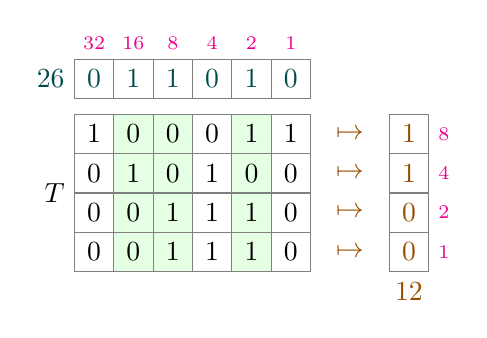
\begin{tikzpicture}[scale=0.5]
\pgfmathsetseed{42}
  \foreach\x in {1,2,4} 
  \filldraw[draw=none, fill=green!10] (\x,0) rectangle (\x+1,-4);
  \foreach \i in {1,...,4} {
    \foreach \j in {1,...,6} {
      \pgfmathtruncatemacro{\b}{Mod(10000*random(),2)}
      \node at (\j-0.5,0.5-\i) {$\b$};
  }}
  \draw[thin,gray] (0,0) grid (6,-4);
  \node[left] at (0,-2) {$T$};
  
  \begin{scope}[shift={(0,0.4)}]
    \draw[thin, gray] (0,0) grid (6,1);
    \node[left,teal!60!black] at (0,0.5) {$26$};
    \foreach\b[count=\x] in{0,1,1,0,1,0}
    \node[teal!60!black] at (\x-0.5,0.5) {$\b$};
    \foreach\b[count=\x] in{32,16,8,4,2,1}
    \node[above,magenta] at (\x-0.5,1) {{\scriptsize\roboto\b}};
  \end{scope}

  \begin{scope}[shift={(8,0)}]
    \foreach \b [count=\i] in {1,1,0,0} {
      \node[orange!60!black] at (-1,0.5-\i) {$\mapsto$};
      \node[orange!60!black] at (0.5,0.5-\i) {$\b$};
    }
    \draw[thin,gray] (0,0) grid (1,-4);
    \foreach\b[count=\x] in{8,4,2,1}
    \node[right,magenta] at (1,0.5-\x) {{\scriptsize\roboto\b}};
    \node[orange!60!black] at (0.5,-4.5) {$12$};
  \end{scope}
\end{tikzpicture}}


\begin{uloha}
  \label{uloha:hasher}
  Naprogramuj triedu \vb{HashFunc}, ktorá ako parameter v konštruktore dostane číslo $b$
  a seed a vyrobí si náhodnú tabuľku $T$. Potom bude mať \prg!int operator()(unsigned long x)!
  ktorý pre dané \vb{x} vráti $T\cdot x$.
\end{uloha}

Keď sme počítali počet kolízií pri hešovaní s náhodnou funkciu, dostali sme sa to takejto 
situácie: mali sme pevne daný prvok \vb{x} a prvok $z_i\not=\vb{x}$ 
a pýtali sme sa, aká je pravdepodobnosť (ak zoberieme úplne náhodnú hešovaciu funkciu),
že $z_i$ sa zahešuje na rovnakú pozíciu ako \vb{x}. Vyšlo nám, že je to $1/n$ a potom všetko 
dobre dopadlo. Preto si teraz predstavme rovnakú situáciu, iba sa pýtame, aká je pravdepodobnosť,
že $h(z_i)=h(\vb{x})$, ak ako hešovaciu funkciu vybereime náhodnú\footnote{%
  opäť si predstavme, že všetky možné tabuľky nahádžeme do vrecka a jednu si vytiahneme} tabuľku $T$.
Keďže $x\not=z_i$, je nejaká pozícia, kde sa ich bitové zápisy líšia. Dajme tomu,
že $i$-ty bit $x$ je $0$ a $i$-ty bit $z_i$ je $1$. 
To znamená, že ak mám hocijakú tabuľku $T$, tak v $T\cdot x$ sa
$i$-ty stĺpec nevyberie, čiže hodnoty v $i$-tom stĺpci výsledok $T\cdot x$ nijak neovplyvňujú.
Rozdeľme si teraz všetky možné tabuľky $T$ do skupín: v jednej skupine budú všetky tabuľky, ktoré
sa líšía iba v $i$-tom stĺpci a všetko ostatné majú rovnaké. V každej skupine je preto $n=2^b$ 
tabuliek\footnote{toľko je rôznych kombinácií núl a jendotiek v $i$-tom stĺpci}. My sa pýtame, koľko
je tabuliek, pre ktoré $T\cdot x=T\cdot z_i$. V každej skupine je hodnota $T\cdot x$ rovnaká
pre všetky tabuľky z tej skupiny, ale hodnoty $T\cdot y$ sú všetky rôzne. To preto, lebo každá zmena 
jedného bitu v $i$-tom stĺpci $T$ zmení príslušný bit vo výsledku $T\cdot z_i$:


\centerline{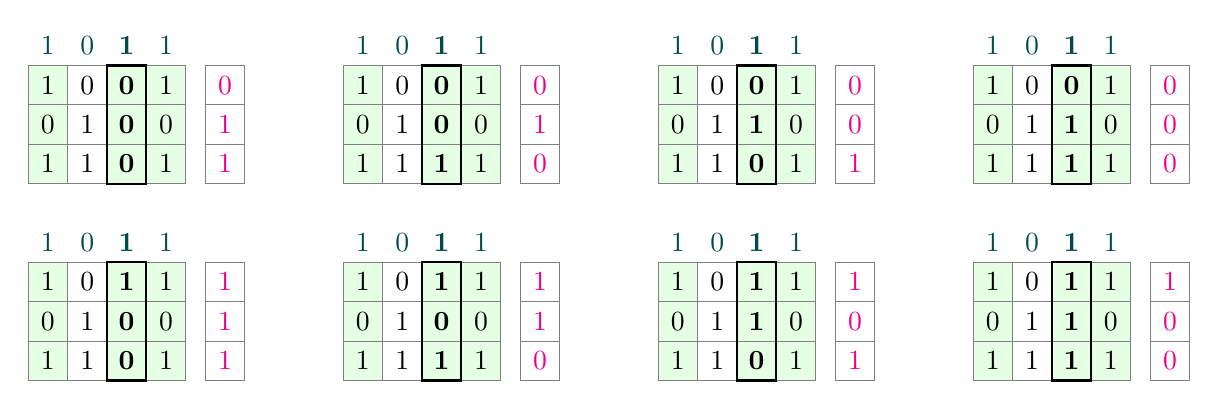
\begin{tikzpicture}[scale=0.5]

\def\base#1{
  \foreach\x in {0,2,3} 
  \filldraw[draw=none, fill=green!10] (\x,0) rectangle (\x+1,-3);
  
  \foreach \x/\v/\b in {0/1/{1,0,1}, 1/0/{0,1,1}, 3/1/{1,0,1}} {
    \node[teal!60!black] at (\x+0.5,0.5) {$\v$}; 
    \foreach \j [count = \y] in \b {
      \node at (\x+0.5,0.5-\y) {$\j$};
    }
  }

  \node [teal!60!black] at (2.5,0.5) {$\mathbf 1$};
  \foreach \i in {0,...,2} {
    \pgfmathtruncatemacro{\tmp}{int(Mod(int(#1/int(2^(2-\i))),2))}
    \node at (2.5,-0.5-\i) {$\mathbf \tmp$};
  }

  \draw[thin,gray] (0,0) grid (4,-3);
  \draw[thick] (2,0) rectangle (3,-3);
  
  \begin{scope}[shift={(4.5,0)}]
    \draw[thin,gray] (0,0) grid (1,-3);
    \foreach \x[count=\i] in {0,1,1} {
      \pgfmathtruncatemacro{\tmp}{int(Mod(\x+int(Mod(int(#1/int(2^(3-\i))),2)),2))}
      \node[magenta] at (0.5,0.5-\i) {$\tmp$};
    }
  \end{scope}
}
  \foreach \x in {0,...,3} \foreach \y in {0,1} {
    \begin{scope}[shift={(8*\x,-5*\y)}]
      \pgfmathtruncatemacro{\p}{\x+4*\y}  
    \base\p
    \end{scope}
  }

\end{tikzpicture}}


Takže z každej skupiny je iba jedna tabuľka $T$, pre ktorú $T\cdot z_i = M\cdot x$, a preto náhodná
tabuľka má pravdepodobnosť $1/n$, že spôsobí kolíziu $z_i$ a $x$. Zvyšok výpočtu prejde rovnako
ako pre úplne náhodné funkcie. 


Preto ak spojíš triedu \vb{HashMap} s výsledkom úlohy~\ref{uloha:hasher}, dostaneš
riešenie úlohy so žiarovkami, kde v priemernom prípade každá operácia prezrie iba konštantne
dlhý zoznam. Oprávnene ale môžeš namietať, že na vyrátanie hešovacej funkcie, t.j. na zránie
$T\cdot\vb{x}$ treba zhruba $\log M\cdot\log n$ operácií, takže sme si oproti vyhľadávaciemu
stromu zase až tak nepomohli. To je pravda, ale dajú sa nájsť podobné sady hešovacích funkcií,
ktoré majú rovnaké vlastnosti, ale dajú sa zrátať rýchlejšie. Napríklad 
ak zoberieme nejaké prvočíslo $p>M$ a náhodnú hešovaciu funkciu urobíme takto: 
zvolíme sí náhodné čísla $a,b$ tak, že $1\le a< p$ a $0\le b< p$ a 
$\vb{h}(x)$ bude $((ax+b) \mod p)\mod n$. Veľmi podobnými, len trochu dlhšími, výpočtami sa dá prísť
na to, že aj táto sada hešovacích funkcií funguje, a navyše sa dá aj rýchlo vyrátať. 


Posledná vec, čo chýba k úplnosti, je znalosť $n$. V úlohe so žiarovkami som zámerne povedal, že je 
dopredu známe, koľko rôznych výrobných čísel sa objaví. V iných úlohách to tak nie je. Dá sa
to však vyriešiť podobne ako v prípade triedy \vb{vector}: budem si sledovať, ako veľmi je moja
hešovacia tabuľka zaplnená, a keď sa zaplní priveľa, zväčším ju a všetky prvky v nej zahešujem
nanovo. Tým sa aj zabezpečí, že ak som mal smolu\footnote{Alebo mi niekto zámerne
zostrojil vstup, v ktorom má moja funkcia veľa kolízií, čo je typický pripad, ak napr. progamuješ
algoritmy na šifrovanie} a niektorý zoznam je príliš dlhý, po prehešovaní očakávam, že sa prvky
rozdelia rovnomerne. 


Môže to celé fungovať?  V STL je trieda \prg!unordered_set!, ktorá sa správa skoro rovnako ako\indexItem{Prg}{\vb{unordered\_set}}
náš starý známy \prg!set!, ale namiesto vyhľadávacieho stromu má hešovaciu tabuľku. To spôsobí,
že iterátor nedáva prvky v utriedenom poradí, a je iba jednosmerný. Ale zase prístup do  
\prg!unordered_set! je o dosť rýchlejší:


%\tikzset{external/force remake}
\begin{tikzpicture}
  \def\plota[#1]#2#3{%
    \addplot[#1,mark=*, 
    line join=round, mark size=0.5pt] table [y=#2, x=n]{data/tree_test2.dat};
    \addlegendentry{\vb{#3}}
  }
  \def\plotb[#1]#2{%
    \addplot[#1, line join=round, mark=none, forget plot,
    name path=#2lo] table [y=#2min, x=n]{data/tree_test2.dat};
    \addplot[#1, line join=round, mark=none, forget plot,
    name path=#2hi] table [y=#2max, x=n]{data/tree_test2.dat};
    \addplot[#1,opacity=0.5,forget plot] fill between[of=#2lo and #2hi];
  }
\begin{axis}[
  width=\textwidth, 
  height=8cm,
  xlabel=$n$,
  ylabel=čas ($\mu$s),
  legend cell align={left},
  legend pos = north west,
  %ymax=0.9,
  %  scaled x ticks=false,
  %scaled y ticks=false,
    /pgf/number format/.cd,
        1000 sep={}
]
%  \plotb[cyan!20]{aa}
%  \plotb[orange!20]{set}
%  \plotb[pink!40]{uset}
  \plota[blue!80]{aa}{aatree.h}
  \plota[orange!80]{set}{set<int>}
  \plota[magenta!80]{uset}{unordered\_set<int>}
\end{axis}
\end{tikzpicture}
%\tikzset{external/force remake=false}


Záverečné poučenie z tejto časti je, že ak nepotrebuješ mať prvky utriedené, je spravidla
niekoľkonásobne rýchlejšie použiť \prg!unoredered_set!, resp. obdobnú \prg!unordered_map!.


Ako všetko v STL, aj \prg!unorederd_set! je šablóna, takže môžeš mať napr. 
\prg!unordered_set<string>!. Ako to ale funguje, keď doposiaľ všetko okolo hešovania
sa dialo na celých číslach? V STL je funkcia, ktorá zo stringu vyráta číslo, a to potom
slúži ako kľúč do hešovacej funkcie. Táto funkcia musí byť tiež starostivo vybraná, lebo
každé dva stringy, ktoré v nej budú mať rovnaký kľúč, skončia vždy v rovnakom zozname v hešovacej 
tabuľke, nech by už hešovacia funkcia bola akokoľvek rafinovaná. Takže ak používaš napr.
\prg!unordered_set<string>!, treba si uvedomiť, že každý prístup znamená prejsť daný string
a zrátať jeho kľúč. 


\prg!unordered_set<string>! je v poriadku, ale keď napíšeš napr. 

\vskip 2ex
\vbox{
\begin{lstlisting}
#include <iostream>
#include <string>
#include <unordered_set>
using namespace std;

struct Clovek {
  string meno;
  int vek;
};

int main() { unordered_set<Clovek> ludia; }
\end{lstlisting}
}

kompilátor vypíše dlhý zoznam chýb, kde sa bude asi medzi iným hovoriť niečo ako\\
\vb{call to implicitly-deleted default constructor of 'unordered\_set<Clovek>'}\\
a možno aj 
\vb{use of deleted function ‘std::hash<Clovek>::hash()’}\\
Tým ti chce povedať, že pre triedu \vb{Clovek} mu chýba práve tá funkcia, ktorá z premennej typu
\vb{Clovek} urobí kľúč do hešovacej tabuľky. Aby si mohol \prg!unordered_set<Clovek>! používať,
treba takú funkciu dodať. Ukážem ti ako, ale na to treba povedať, čo je to tzv. {\em špecializácia
šablóny}.


Dajme tomu, že mám takúto šablónu \indexItem{Prg}{špecializácia šablóny}

\vskip 2ex
\begin{lstlisting}
template <typename T>
struct Vec {
  T x;
  void daj() { cout << "mam vec, ale neviem, co s nou" << endl; }
};
\end{lstlisting}

V programe môžem napísať

\begin{lstlisting}
Vec<int> a; 
Vec<string> b; 
a.x = 42;
b.x = "dvaastyridsat";
a.daj();
b.daj();
\end{lstlisting}

Tým hovorím kompilátoru, aby si zo šablóny vyrobil dva (z pohľadu ďalšieho programu
úplne nezávislé) typy \prg!Vec<int>!
a \prg!Vec<string>!, vyrobil príslušné premenné atď, a keď to spustím, dvakrát sa vypíše tá istá veta.
Niekedy sa ale hodí urobiť výnimku a povedať kompilátoru napr. \cmd{''Všetky typy  
\prg!Vec<string>!, \prg!Vec<bool>!, atď. \ rob podľa šablóny, ale typ \prg!Vec<int>! urob
inak''}. Takáto výnimka sa volá špecializácia a viem ju napísať takto:

\vskip 2ex
\begin{lstlisting}
template <typename T>
struct Vec {
  T x;
  void daj() { cout << "mam vec, ale neviem, co s nou" << endl; }
};

template <>
struct Vec<int> {
  int a;
  Vec(int x, int y) { a = x + y; }
  void daj() { cout << "mam int " << a << endl; }
};
\end{lstlisting}

Zátvorky v \prg!template! ostanú prázdne a za meno typu dosadím parameter, ktorý špecializujem. Takto 
vyrobený typ nemá s pôdovným nič spoločmé, môže mať iné premenné aj metódy. Často je ale
rozumné mať (aj) metódy, čo sa volajú rovnako. Teraz by som mohol napísať

\begin{lstlisting}
Vec<int> a(5,6); 
Vec<string> b; 
b.x = "dvaastyridsat";
a.daj();
b.daj();
\end{lstlisting}

a program by vypísal:

\begin{outputBox}
mam int 11
mam vec, ale neviem, co s nou
\end{outputBox}



Niekedy chcem pri špecializácii zmeniť len zopár detailov a 
chcem, aby väčšina vecí ostala rovnaká, ako v šablóne. V tom prípade môžem špecializovať iba 
jednotlivé metódy takto:\indexItem{Prg}{\vb{struct std::hash}}

\begin{lstlisting}
template <>
void Vec<int>::daj() {cout << "mam int " << x << endl; }
\end{lstlisting}

Opäť začínam prázdnym 
\prg!template <>! a potom nasleduje funkcia, ktorú chcem zmeniť. Musím ale povedať, komu
patrí, a to robím dvoma dvojbodkami. V tomto prípade hovorím \cmd{'' Typ \prg!Vec<int>!
urob podľa šablóny, ale jeho metódu \prg!daj()! urob takto.''}


Funkcia, ktorá pre rôzne typy hovorí, ako vyrobiť kľúč do hešovacej funkcie je v STL
urobená cez triedu \prg!hash!. Je to jednoduchá šablóna, ktorá vyzerá zhruba takto

\begin{lstlisting}
template <typename Key>
struct hash {
  unsigned long operator()(const Key &x) const { ... }
};
\end{lstlisting}

To znamená, že premenná \prg!hash<T> h! má operátor \prg!h(x)!, ktorý zoberie premennú typu 
\prg!T! a vráti jej hešovací kľúč. Môžeš si to vyskúšať, 

\vskip 2ex
\begin{lstlisting}
hash<string> h;
cout << h("hrom do toho") << endl;
\end{lstlisting}

vypíše napr. \vb{14868293708368628758}. Funkcie v \prg!unordered_map! a \prg!unordered_set!
používajú príslušný typ \prg!hash! na to, aby vyrobili hešovacie kľúče. Samotná šablóna
\vb{hash} je naprogramovaná tak, aby spôsobila chybu, všetku prácu musia robiť jej 
výnimky-špecializácie. Keď chcem používať \prg!unordered_set<Clovek>!, musím\footnote{%
no nemusím, sú aj iné možnosti, ale o nich tu teraz nehovorím} preto
dodať špecializáciu \prg!hash<Clovek>!. To môžem spraviť napr. takto:

\vbox{
\begin{lstlisting}
template <>
struct std::hash<Clovek> {
  unsigned long operator()(const Clovek& c) const {
    return 42;
  }
};
\end{lstlisting}
}

Toto by malo byť jasné, jediná vec, čo stojí za pozornosť je, že nakoľko \prg!hash! patrí do
 \prg!namespace std!, tak pri špecializácii musím napísať celé
meno \prg!std::hash! aj keď som si na začiatku ''privlastnil'' všetko zo \prg!std! pomocou
\prg!using namespace std;!.


Hešovacia tabuľka v knižnici \prg!<unordered_map>! potrebuje okrem rátania kľúča objekty porovnávať,
preto do triedy \vb{Clovek} treba pridať operátor \prg!==!

\begin{lstlisting}
struct Clovek {
  string meno;
  int vek;
  bool operator==(const Clovek& c) const {
    return meno == c.meno && vek == c.vek;
  }
};
\end{lstlisting}


Teraz sa program, ktorý používa \prg!unordered_set<Clovek>! bude dať skompilovať aj spustiť,
len namiesto hešovacej tabuľky budem mať len spájaný zoznam: všetky premenné dostanú rovnaký kľúč
$42$, a tak sa vždy zahešujú na to isté miesto, kde vznikne dlhý zoznam. 
Ako môžem získať rozumný kľúč? To je celkom na dlhú diskusiu, ale na bežné účely poslúži aj
jednoduchý prístup: ak \prg!string! a \prg!int! už majú dobré špecializácie \prg!hash!, tak 
ja len vrátim ich \vb{XOR}

\begin{lstlisting}
template <>
struct std::hash<Clovek> {
  unsigned long operator()(const Clovek& c) const {
    return hash<string>()(c.meno) ^ hash<int>()(c.vek);
  }
};
\end{lstlisting}

Čo je to za zápis? \prg!hash<string>()! je volanie konštruktora, t.j. vyrobí 
premennú typu \prg!hash<string>!. Vzápätí zavolám jej \prg!operator()(const string &x)!
s parametrom \prg!c.meno! a dostanem nejaké číslo typu \prg!unsigned long!. Dočasnú premennú
typu \prg!hash<string>! potom zahodím. Rovnako sa to urobí pre \prg!hash<int>!. Takže nakoniec
mám dve čísla, z ktorých urobím bitový \vb{XOR} (\prg!^!).

